\documentclass[11pt,a4paper]{article}

\usepackage[T1]{fontenc}
\usepackage{lmodern}
\usepackage[margin=2.5cm]{geometry}
\usepackage{amsmath,amssymb,amsthm,bm}
\usepackage{booktabs,tabularx,array}
\usepackage{graphicx}
\usepackage{float}
\usepackage{xcolor}
\usepackage{listings}
\usepackage{tikz}
\usetikzlibrary{arrows.meta,positioning,shapes.geometric}
\usepackage{microtype}
\usepackage{enumitem}
\usepackage[hidelinks]{hyperref}

\theoremstyle{definition}
\newtheorem{definition}{Definition}[section]
\theoremstyle{remark}
\newtheorem{remark}{Remark}[section]

\newcommand{\x}{\mathbf{x}}
\newcommand{\R}{\mathbb{R}}
\newcommand{\ind}{\mathbb{1}}
\DeclareRobustCommand{\code}[1]{\texttt{\detokenize{#1}}}
\pdfstringdefDisableCommands{\def\code#1{#1}}
\newcolumntype{Y}{>{\raggedright\arraybackslash}X}

\definecolor{codebg}{gray}{0.96}
\lstset{
  language=Python,
  basicstyle=\ttfamily\small,
  backgroundcolor=\color{codebg},
  frame=single, rulecolor=\color{gray!40},
  keywordstyle=\color{blue!60!black}\bfseries,
  commentstyle=\color{green!40!black}\itshape,
  stringstyle=\color{red!50!black},
  columns=fullflexible, keepspaces=true,
  breaklines=true, showstringspaces=false,
  xleftmargin=4pt, xrightmargin=4pt, aboveskip=8pt, belowskip=8pt
}

\title{Niching Subset Simulation:\\ an Implementation Guide and User Manual}
\author{Companion notes to the single-file implementation}
\date{15 October 2026}

\begin{document}
\maketitle

\begin{abstract}
These notes document a single Python program that estimates small failure probabilities
$p_F = P\big(g(\x) \ge Y_F\big)$, $\x \sim N(\mathbf{0}, \mathbf{I}_d)$, with two methods side by side:
a vectorised implementation of subset simulation (SuS) in the sense of Au and Beck~\cite{aubeck},
and Kinnear's niching subset simulation (NSuS)~\cite{kinnear}, copied verbatim from the authors'
companion repository. We describe every component of the code, state the mathematics each
component implements, explain every figure the program produces, and show how to change the
performance function and the algorithmic parameters for experiments. Numerical results are
reported for the ring problem $g(\x) = x_1^2 + x_2^2$ and for the piecewise linear example of~\cite{kinnear}.
\end{abstract}

\tableofcontents
\newpage

%=====================================================================
\section{Introduction}
%=====================================================================

Let $\x = (x_1, \dots, x_d)$ have independent standard normal components, let
$g : \R^d \to \R$ be a \emph{performance function} and $Y_F$ a \emph{critical threshold}. The
\emph{failure domain} and \emph{failure probability} are
\begin{equation}\label{eq:pf}
F = \{\x \in \R^d : g(\x) \ge Y_F\}, \qquad p_F = P(\x \in F) = \int_{\R^d} \ind_F(\x)\, \varphi_d(\x)\, d\x ,
\end{equation}
where $\varphi_d$ is the $d$-dimensional standard normal density. When $p_F$ is of order
$10^{-4}$ or smaller, crude Monte Carlo needs roughly $10/p_F$ evaluations of $g$ to observe
ten failures. Subset simulation reduces this cost by writing $F$ as the last of a nested sequence
of more probable events. Its weakness is that the sequence follows a \emph{single} path; if
$F$ consists of several separate regions, regions that look unpromising early may be lost.
Niching subset simulation grows a \emph{tree} of levels instead, and follows each region
(\emph{niche}) on its own branch.

\subsection{Layout of the program}

The program is one Python file. Table~\ref{tab:layout} lists its parts in file order and their origin.

\begin{table}[H]
\centering
\small
\begin{tabularx}{\textwidth}{@{}l Y l@{}}
\toprule
Part & Content & Origin \\
\midrule
Imports & numerical, graph, machine-learning and plotting libraries & both \\
Parameters & $d$, $Y_F$, $n$, $p$, \code{SEED}, \code{SAVE_PLOT}, \code{GRAPH_SIZE}, \code{MAX_BRANCHES}, \code{SCALE} & user \\
\code{performance_function} & $g$; currently $g(\x) = x_1^2 + x_2^2$ & user \\
\code{subset_simulation} & subset simulation, Section~\ref{sec:sus} & user \\
\code{verbose} \dots{} \code{HillValleyGraphNSuS} & the NSuS package, Sections~\ref{sec:blocks}--\ref{sec:estimate} & Kinnear, verbatim \\
\code{plot_levels_2d} & Figure~\ref{fig:sus} & user \\
\code{plot_nsus_levels_2d}, \code{plot_branch_tree} & Figures~\ref{fig:niches}, \ref{fig:tree} & added \\
\code{contour_plot}, \code{partitioner_figures} & Figures~\ref{fig:graphsamples}--\ref{fig:classifier} & Kinnear's figure scripts \\
run block & runs both methods, prints, plots & user, plus Kinnear's example \\
\bottomrule
\end{tabularx}
\caption{The parts of the program.}\label{tab:layout}
\end{table}

%=====================================================================
\section{Problem set-up}\label{sec:setup}
%=====================================================================

\subsection{Parameters}

\begin{lstlisting}
d = 2              # dimension of the input space
YF = 20.0          # critical threshold (failure <=> g(x) > YF)
n = 3000           # number of samples per level
p = 0.1            # level probability
SEED = 0           # integer for repeatable results, None for random
SAVE_PLOT = None   # e.g. "levels.png" to save Figure 1

GRAPH_SIZE = 15    # NSuS: samples in each hill valley graph
MAX_BRANCHES = 4   # NSuS: maximum number of branches (1 = plain SuS)
SCALE = 1.0        # NSuS: proposal std of the Markov chains (None = adaptive)
\end{lstlisting}

\subsection{The performance function}

\begin{lstlisting}
def performance_function(x):
    return np.sum(x**2, axis=0)
\end{lstlisting}

This is the \emph{ring} problem,
\begin{equation}
g(\x) = x_1^2 + x_2^2, \qquad F = \{\x : \|\x\| \ge \sqrt{Y_F}\},
\end{equation}
a failure domain with no single most probable point. Since $\|\x\|^2 \sim \chi^2_d$, the exact answer is
\begin{equation}\label{eq:chi2}
p_F = P(\chi^2_d \ge Y_F) \overset{d=2}{=} e^{-Y_F/2}, \qquad Y_F = 20:\; p_F = e^{-10} \approx 4.54\times 10^{-5},
\end{equation}
which the run block computes as \code{chi2.sf(YF, d)}.

\begin{remark}[Two input shapes]
The function is called with a $(d, N)$ array by subset simulation and the plots, and with a single
point by Kinnear's code. Summing over \code{axis=0} serves both. Kinnear's code passes the point
as a Python \emph{tuple} (so that it can be a dictionary key, Section~\ref{sec:cache}); the run block
therefore hands NSuS the wrapper
\begin{center}\code{lambda x: performance_function(np.array(x))}.\end{center}
\end{remark}

%=====================================================================
\section{Subset simulation}\label{sec:sus}
%=====================================================================

\subsection{Principle}

Choose thresholds $Y_1 < Y_2 < \dots < Y_L < Y_F$ and write $F_k = \{g(\x) > Y_k\}$, so that
$F_1 \supset F_2 \supset \dots \supset F_L \supset F$. Then
\begin{equation}\label{eq:sus}
p_F = P(F_1) \prod_{k=2}^{L} P(F_k \mid F_{k-1}) \; P(F \mid F_L).
\end{equation}
The thresholds are chosen adaptively so that every factor except the last equals $p$ (here $0.1$),
which can be estimated accurately from a moderate number of samples.

\subsection{Algorithm}

Let $n_c = np$ be the number of Markov chains and $n_s = (1-p)/p$ the number of new states per chain,
so that $n = n_c(n_s + 1)$; with $n = 3000$, $p = 0.1$ this is $3000 = 300 \times 10$.

\begin{enumerate}[label=\textbf{Step \arabic*.}, leftmargin=*]
\item \emph{Level 0.} Draw $\x^{(1)}, \dots, \x^{(n)} \sim N(\mathbf{0}, \mathbf{I}_d)$, evaluate
$y^{(i)} = g(\x^{(i)})$ and count $n_F = \#\{i : y^{(i)} > Y_F\}$.
\item \emph{Stopping rule.} If $n_F / n \ge p$, stop.
\item \emph{Threshold and seeds.} Sort the level so that $y_{(1)} \ge \dots \ge y_{(n)}$ and set
\begin{equation}
Y_L = \tfrac12\big(y_{(n_c)} + y_{(n_c+1)}\big).
\end{equation}
The $n_c$ samples above $Y_L$ are the \emph{seeds}; they are distributed as $\varphi_d(\cdot \mid F_L)$.
\item \emph{Modified Metropolis.} From each seed $\mathbf{z}^{(0)}$ run $n_s$ steps. Given
$\mathbf{z}^{(m)}$, for every coordinate $j$ propose $\xi_j = z_j^{(m)} + \varepsilon_j$,
$\varepsilon_j \sim N(0,1)$, and set
\begin{gather}
q_j = \begin{cases} \xi_j & \text{with probability } \min\!\big(1, \varphi(\xi_j)/\varphi(z_j^{(m)})\big), \\ z_j^{(m)} & \text{otherwise}, \end{cases}
\\
\mathbf{z}^{(m+1)} = \begin{cases} \mathbf{q} & \text{if } g(\mathbf{q}) > Y_L, \\ \mathbf{z}^{(m)} & \text{otherwise.} \end{cases}
\end{gather}
The coordinate-wise acceptance preserves $\varphi_d$; the second test keeps the chain in $F_L$.
\item The $n_c(n_s+1) = n$ states form the next level; return to Step 2.
\end{enumerate}

\subsection{Estimate and cost}

After $L$ conditional levels,
\begin{equation}
\hat p_F^{\,\mathrm{SS}} = p^{L}\, \frac{n_F}{n}, \qquad N = n + n(1-p)L .
\end{equation}
The function returns a dictionary with keys \code{pF_SS}, \code{N}, \code{L}, \code{Y},
\code{nF}, \code{x} and \code{y}.

\begin{remark}
(i) Only one path is followed, so a failure region whose samples are not among the best
$100p\,\%$ at some level is lost. (ii) If all chains are trapped on a local maximum of $g$ below
$Y_F$, the thresholds stop rising and the loop in Step 2 does not terminate; Section~\ref{sec:trouble} gives a guard.
\end{remark}

%=====================================================================
\section{The building blocks of NSuS}\label{sec:blocks}
%=====================================================================

Kinnear's implementation is a set of small classes. Each is listed below with the file of the
\code{nsus/} package it comes from.

\subsection{Cached performance function (\code{performance_function.py})}\label{sec:cache}

\begin{lstlisting}
def __call__(self, x):
    tuple_x = tuple(x)
    try:
        result = self.cache[tuple_x]
    except KeyError:
        self.cache[tuple_x] = result = self.non_cache_performance_function(tuple_x)
    return result
\end{lstlisting}
Every evaluation is stored in the dictionary $\mathcal{H}$ (\code{cache}), the \emph{search history}.
The cost reported for NSuS is $N = |\mathcal{H}|$ (\code{eval_count}), the number of \emph{distinct}
points evaluated; repeated states of a Markov chain are free.

\subsection{Samples and indicators (\code{level_create.py}, \code{indicator.py})}

A \code{Sample} is a pair $(\x, g(\x))$.

\begin{definition}[Indicator]
An indicator with threshold $b$ and niche function $\ind_A$ is
\begin{equation}
I(\x) = \ind_A(\x)\, \ind\{g(\x) \ge b\}.
\end{equation}
Its method \code{child_indicator}$(b', \ind_{A'})$ returns the indicator
$\ind_A(\x)\ind_{A'}(\x)\ind\{g(\x) \ge b'\}$, and \code{new_threshold}$(b')$ returns
$\ind_A(\x)\ind\{g(\x) \ge b'\}$.
\end{definition}
Hence the region of a level at depth $m$ on a branch with niches $A_1, \dots, A_m$ is
\begin{equation}
R_m = \Big(\bigcap_{k=1}^{m} A_k\Big) \cap \{g \ge b_m\},
\end{equation}
so niches nest: a branch never leaves the niches of its ancestors.

\subsection{Markov chain (\code{markov_chain.py})}

\code{ModifiedMetropolis.update} implements Step~4 of Section~\ref{sec:sus} in logarithmic form,
\begin{equation}
\text{accept } \xi_j \iff \log\varphi(\xi_j) - \log\varphi(z_j) \ge \log u_j, \quad u_j \sim U(0,1),
\end{equation}
with proposal standard deviation $\sigma_j$ supplied by a \emph{scaler}, and with the region test
$I(\mathbf{q}) = 1$ in place of $g(\mathbf{q}) > Y_L$. The \code{ConstantScaler} uses $\sigma_j = $ \code{SCALE};
the \code{AdaptiveScaler} (\code{SCALE = None}) uses the sample standard deviation of the seeds in coordinate $j$.

\subsection{Buds (\code{bud_create.py})}

\begin{definition}[Bud]
A \emph{bud} is a level that has been specified but not yet sampled: a set of seeds, an indicator $I$,
a scale $\sigma$ and a parent level. It is \emph{used} once it has been grown into a level.
\end{definition}

Given a level $L$ with $|L|$ samples and a niche $A$, \code{BudCreator.create} forms
\begin{align}
\text{candidates } C &= \{\x \in L : \ind_A(\x) = 1\}, \text{ sorted by } g, \\
\text{seeds } S &= \text{the best } \min\big(\lfloor p|L| \rfloor, |C|\big) \text{ elements of } C, \\
\text{threshold } b' &= \min_{\x \in S} g(\x).
\end{align}
Every level receives a \emph{trivial bud} with $A = \R^d$ (the SuS continuation, used by the
stopping rules); a level that is split receives one bud per niche, stored in \code{_buds}.

\subsection{Levels (\code{level.py})}

A \code{Level} is a node of an \code{anytree} tree. Its \code{name} is the number of levels in the
tree at the moment it is created, so names are $1, 2, 3, \dots$ in creation order. Further members
are listed in Table~\ref{tab:level}.

\begin{table}[H]
\centering\small
\begin{tabularx}{\textwidth}{@{}l Y@{}}
\toprule
Member & Meaning \\
\midrule
\code{chain_list}, \code{sample_list}, \code{level_size} & samples by chain, flattened, and their number $|L|$ \\
\code{indicator} & the region $R$ the level was sampled from \\
\code{buds} & \code{_buds} if the level was split, otherwise the trivial bud \\
\code{branch} & the path from the root to the level \\
\code{stop_info} & which stopping rules fired \\
\code{non_used_buds} & all unused buds in the whole tree \\
\code{non_used_non_stop_buds} & those whose parent level has not stopped (the options) \\
\code{extra_info} & graph, communities and classifier saved by the partitioner \\
\bottomrule
\end{tabularx}
\caption{Members of \code{Level}.}\label{tab:level}
\end{table}

\subsection{Allocation, choice and stopping}

\paragraph{Allocator (\code{allocate.py}).} \code{SubsetAllocator} uses chains of length $1/p$.
\code{BranchingAllocator}, used by NSuS, divides the budget $\lfloor n(1-p)\rfloor$ among the
$B$ buds open at the time:
\begin{equation}\label{eq:alloc}
\ell = \left\lfloor \frac{\lfloor n(1-p)\rfloor}{B\,|S|} \right\rfloor + 1, \qquad |L_{\text{new}}| = |S|\,\ell .
\end{equation}

\paragraph{Chooser (\code{choose.py}).} \code{DepthChooser} grows an open bud whose parent level has
minimal depth. The tree is therefore grown one depth at a time.

\paragraph{Stopping (\code{stop.py}).} With $b'$ the threshold of the trivial bud and $b$ that of the level,
\begin{equation}
\text{Failure:}\ b' \ge Y_F, \qquad \text{ThresholdConverge:}\ b' \le b .
\end{equation}
The first means at least $\lfloor p|L|\rfloor$ samples already fail; the second means the branch has
stopped making progress. A stopped level is the end of its branch.

%=====================================================================
\section{The main loop}\label{sec:loop}
%=====================================================================

\begin{lstlisting}
def run(self):
    while not self.is_stop:
        if self.is_initial:
            self.initial_level = self.level_creator.create_initial()
            level = self.initial_level
        else:
            bud = self.chooser.choose(self.options)
            level = self.level_creator.create(bud)
        self.bud_creator.create_trivial(level)
        self.stopper.stop(level)
        if not level.is_stop:
            partition_indicators = self.partitioner.partition(level)
            if len(partition_indicators) > 1:
                self.bud_creator.create_inidicator_buds(level, partition_indicators)
    self.print_terminate()
\end{lstlisting}

\begin{figure}[h]
\centering
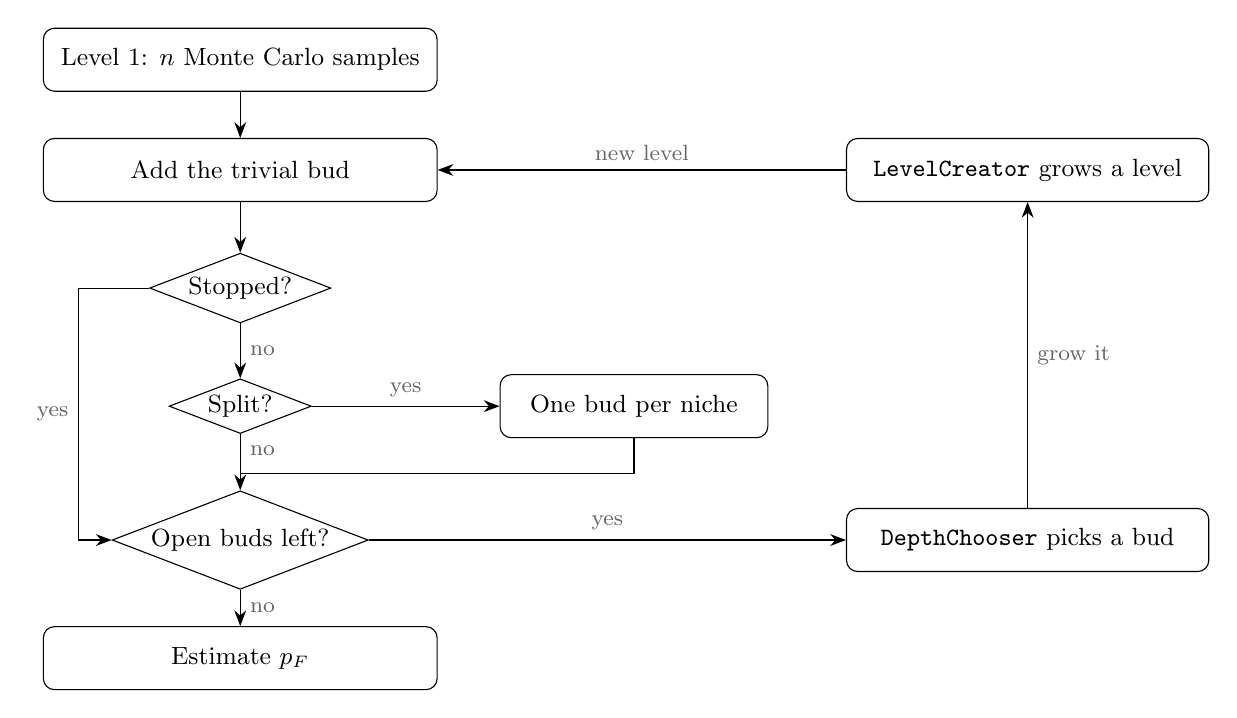
\begin{tikzpicture}[
  box/.style={draw, rounded corners, minimum height=8mm, align=center, font=\small},
  dec/.style={draw, diamond, aspect=2.6, inner sep=1pt, align=center, font=\small},
  arr/.style={-{Stealth[length=2mm]}},
  lab/.style={font=\footnotesize, text=black!60}]
\node[box, minimum width=50mm] (init)  at (0, 0)    {Level 1: $n$ Monte Carlo samples};
\node[box, minimum width=50mm] (triv)  at (0,-1.4)  {Add the trivial bud};
\node[dec]                     (stop)  at (0,-2.9)  {Stopped?};
\node[dec]                     (split) at (0,-4.4)  {Split?};
\node[box, minimum width=34mm] (niche) at (5.0,-4.4) {One bud per niche};
\node[dec]                     (open)  at (0,-6.1)  {Open buds left?};
\node[box, minimum width=50mm] (fin)   at (0,-7.6)  {Estimate $p_F$};
\node[box, minimum width=46mm] (choose) at (10,-6.1) {\code{DepthChooser} picks a bud};
\node[box, minimum width=46mm] (grow)  at (10,-1.4) {\code{LevelCreator} grows a level};
\draw[arr] (init) -- (triv);
\draw[arr] (triv) -- (stop);
\draw[arr] (stop) -- node[lab, right]{no} (split);
\draw[arr] (stop.west) -- ++(-0.9,0) |- node[lab, pos=0.25, left]{yes} (open.west);
\draw[arr] (split) -- node[lab, above]{yes} (niche);
\draw[arr] (split) -- node[lab, right, pos=0.3]{no} (open);
\draw (niche.south) |- (0,-5.25);
\draw[arr] (open) -- node[lab, right]{no} (fin);
\draw[arr] (open) -- node[lab, above]{yes} (choose);
\draw[arr] (choose) -- node[lab, right]{grow it} (grow);
\draw[arr] (grow) -- node[lab, above]{new level} (triv);
\end{tikzpicture}
\caption{One pass of \code{NSuS.run} per new level.}\label{fig:loop}
\end{figure}

\begin{remark}[Level sizes]
By~\eqref{eq:alloc}, levels are smaller when more buds are open. In the ring run ($n = 3000$):
levels 2 and 3 have $|S| = 300$, $B = 3$, $\ell = 4$, size $1200$; level 4 has $B = 4$, $\ell = 3$, size $900$;
all later levels have $|S| \in \{120, 90\}$, $B = 4$, $\ell \in \{6, 8\}$, size $720$.
\end{remark}

%=====================================================================
\section{The niching step}\label{sec:niching}
%=====================================================================

\code{HillValleyGraphPartitioner.partition(level)} returns a list of niche functions; a list of length
one means \emph{do not split}. It proceeds in five stages.

\paragraph{Stage 0: admissibility.} With $B$ the number of open buds in the tree,
\begin{equation}
B \ge \texttt{MAX\_BRANCHES} \implies \text{no split}, \qquad k_{\max} = \texttt{MAX\_BRANCHES} - B + 1 .
\end{equation}

\paragraph{Stage 1: graph samples.} The chains of the level are grouped by their seed; within and
across groups the order is randomised, and points are taken one per group in rotation until
$m = \lfloor \texttt{GRAPH\_SIZE}/B \rfloor$ graph samples $\x_1, \dots, \x_m$ are chosen.

\paragraph{Stage 2: hill valley graph.}
\begin{definition}[Hill valley test with history]
For a pair $(i, j)$ let $Q_{ij} = [\min(\x_i, \x_j), \max(\x_i, \x_j)]$ be the axis-aligned box they span,
and $\mathcal{H}_{ij} = \mathcal{H} \cap Q_{ij}$ the stored points inside it, excluding the graph samples.
If $\mathcal{H}_{ij} = \emptyset$, $g$ is evaluated once at $(\x_i + \x_j)/2$ and the point is added to $\mathcal{H}$. Then
\begin{equation}
(i, j) \in E \iff g(\mathbf{h}) \ge \min\big(g(\x_i), g(\x_j)\big) \quad \forall\, \mathbf{h} \in \mathcal{H}_{ij}.
\end{equation}
\end{definition}
An edge means no valley was found between the two points: they appear to lie on the same hill of $g$.
The midpoint evaluations are the only additional cost of NSuS (\code{partitioner.eval_count}).

\paragraph{Stage 3: communities.} Asynchronous label propagation is run $100$ times on $G = (V, E)$.
If more than $50$ of the runs return a single community, the level is not split. Otherwise the
single-community results are discarded and each remaining partition is reduced to at most $k_{\max}$
parts by randomly merging pairs (\code{shrink_partition}).

\paragraph{Stage 4: classifier.} A pipeline \emph{standardise} $\to$ \emph{PCA} (both fitted on all
samples of the level) $\to$ \emph{linear SVC} ($\ell_1$ penalty, $C = 1$) is fitted to each candidate
partition, labelling graph sample $\x_i$ by its community. The partition with the highest balanced
accuracy is kept. The decision boundaries are hyperplanes.

\paragraph{Stage 5: niche functions.} For community label $k$ the niche function is
\begin{equation}
\ind_{A_k}(\x) = \ind\{\text{classifier}(\x) = k\},
\end{equation}
and \code{create_inidicator_buds} creates one bud per niche as in Section~\ref{sec:blocks}.

%=====================================================================
\section{Estimation}\label{sec:estimate}
%=====================================================================

\subsection{The estimator}

For a level $L$ and indicator $I$ let $\hat P(I, L) = |L|^{-1} \sum_{\x \in L} I(\x)$
(\code{probability_of_indicator}). For a branch $L_0 \to L_1 \to \dots \to L_m$ with level indicators
$I_1, \dots, I_m$,
\begin{equation}\label{eq:branch}
\hat p_{\text{branch}} = \prod_{k=1}^{m} \hat P(I_k, L_{k-1}) \cdot \hat P\big(I_m^{Y_F}, L_m\big),
\end{equation}
where $I_m^{Y_F}$ is $I_m$ with its threshold replaced by $Y_F$ (\code{new_threshold}). Without
splitting, each factor is approximately $p$ and~\eqref{eq:branch} reduces to $p^{L} n_F / n$. After a split,
each child's factor counts only its own niche, so the factors of sibling branches sum to approximately
the factor of an unsplit step. The NSuS estimate is the sum over the leaves of the (trimmed) tree,
\begin{equation}\label{eq:nsus}
\hat p_F^{\,\mathrm{NSuS}} = \sum_{\ell \in \text{leaves}} \hat p_\ell
\qquad (\code{exceedance_probability}).
\end{equation}
For the ring run of Section~\ref{sec:run},
\begin{equation}
\hat p_F^{\,\mathrm{NSuS}} = 9.76\times10^{-6} + 1.19\times10^{-5} + 2.69\times10^{-6} + 0 = 2.43\times10^{-5},
\end{equation}
the zero being the branch stopped by ThresholdConverge.

\subsection{Coefficient of variation}

With $P_k = \hat P(I_k, L_{k-1})$,
\begin{equation}
\delta_1 = \sqrt{\frac{1-P_1}{n P_1}}, \qquad
\delta_k = \sqrt{\frac{1-P_k}{|L_{k-1}| P_k}\,(1+\gamma_k)}, \qquad
\delta_{\text{branch}} = \Big(\sum_k \delta_k^2\Big)^{1/2},
\end{equation}
where $\gamma_k$ is the correlation factor of the Markov chains~\cite{aubeck}, estimated from the
auto-correlation of the indicator sequence along each chain (\code{level_gamma}). The branches are combined as
\begin{equation}
\delta_{p_F} = \Big(\sum_{i,j} w_{ij}\,\delta_{a(i,j)}^2\Big)^{1/2}, \qquad
w_{ij} = \frac{\hat p_i \hat p_j}{\sum_{i,j} \hat p_i \hat p_j},
\end{equation}
with $a(i,j)$ the last common ancestor of leaves $i$ and $j$ (\code{cov}). The reliability index is
$\beta = -\Phi^{-1}(p_F)$.

\subsection{The two assembled algorithms}

\begin{table}[H]
\centering\small
\begin{tabularx}{\textwidth}{@{}l Y Y@{}}
\toprule
Component & \code{SubsetSimulation} & \code{HillValleyGraphNSuS} \\
\midrule
Stopping & Failure, ThresholdConverge & same \\
Chooser & \code{DepthChooser} & same \\
Markov chain & \code{ModifiedMetropolis} & same \\
Scaler & constant, or adaptive if \code{scale=None} & same \\
Partitioner & \code{NoPartitioner} (never splits) & hill valley graph, $100$ iterations \\
Classifier & none & $\ell_1$ linear SVC, $C = 1$ \\
Allocator & \code{SubsetAllocator} & \code{BranchingAllocator} \\
\bottomrule
\end{tabularx}
\caption{Kinnear's two assemblies of the \code{NSuS} framework.}
\end{table}

Both share a single random generator \code{np.random.default_rng(seed)}, so a fixed \code{SEED}
reproduces a run exactly.

%=====================================================================
\section{Figures}\label{sec:figures}
%=====================================================================

For $d = 2$ the run block produces seven figures. Those below were produced by the program with the
parameters of Section~\ref{sec:setup}; for Figures~\ref{fig:graphsamples}--\ref{fig:classifier} the axis range
was widened to $[-4.5, 4.5]^2$ and four niche colours were enabled (Section~\ref{sec:change}).

\begin{figure}[p]
\centering
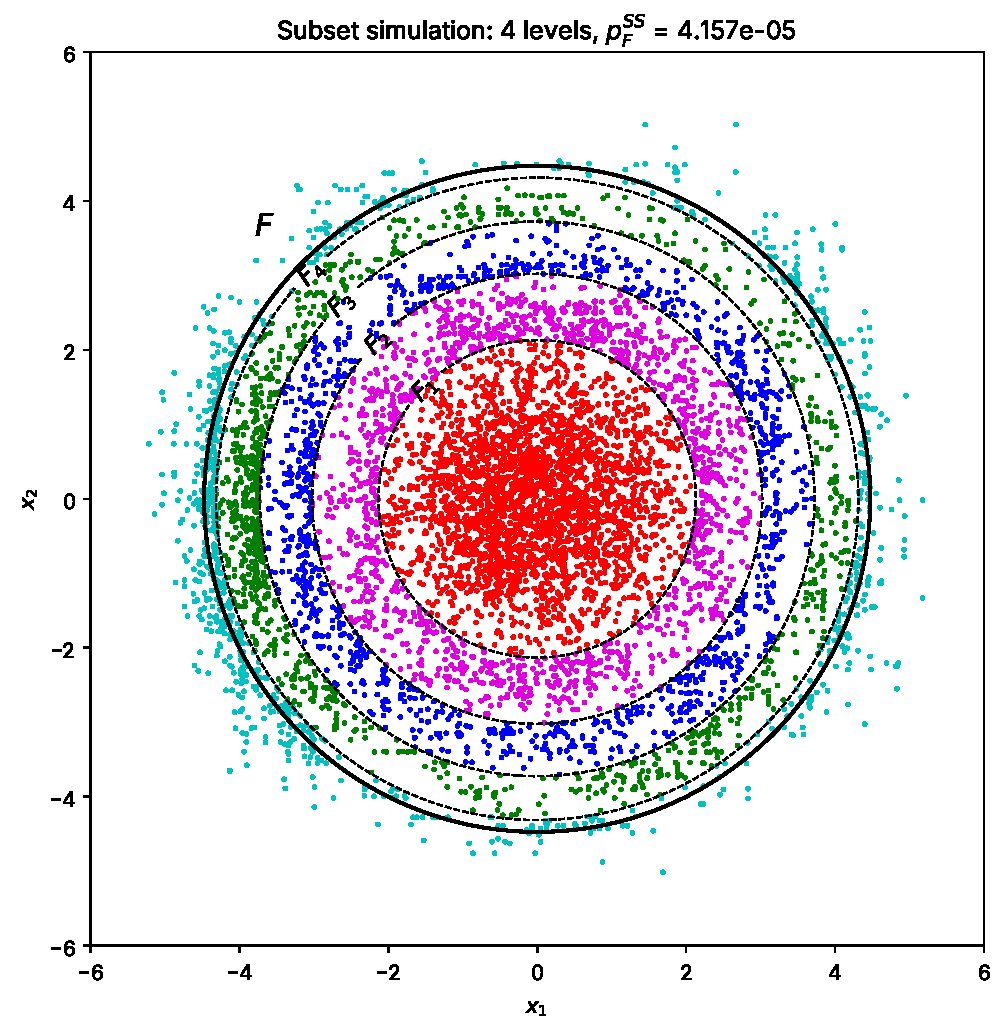
\includegraphics[width=0.62\textwidth]{figures/fig1_sus.pdf}
\caption{Subset simulation (\code{plot_levels_2d}). Samples of each level; dashed curves are the
intermediate thresholds $\{g = Y_L\}$, labelled $F_L$; the solid curve is the failure boundary
$\{g = Y_F\}$.}\label{fig:sus}
\end{figure}

\begin{figure}[p]
\centering
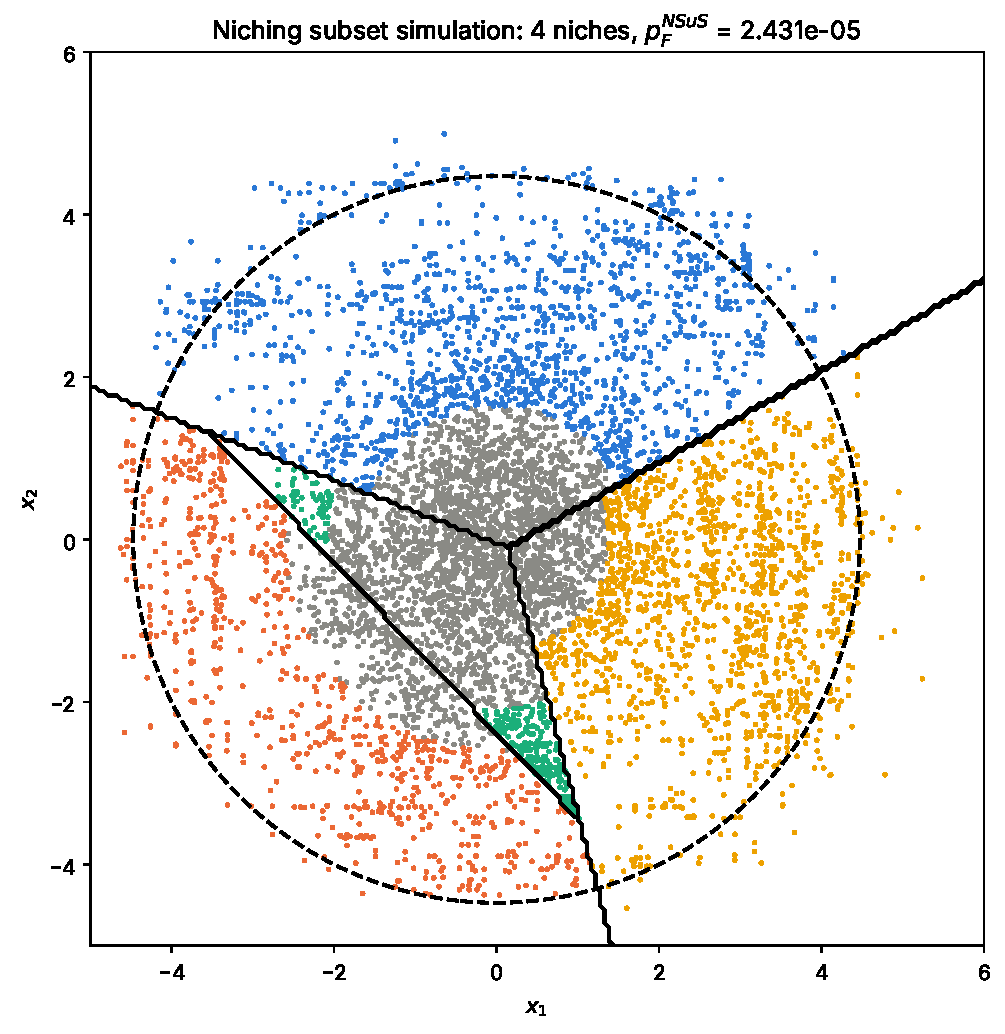
\includegraphics[width=0.62\textwidth]{figures/fig2_niches.pdf}
\caption{NSuS samples by niche (\code{plot_nsus_levels_2d}). Grey: levels before the first split;
colours: branches. Solid lines: classifier boundaries of each split, drawn only inside the region of
the level that was split. Dashed: the failure boundary.}\label{fig:niches}
\end{figure}

\begin{figure}[p]
\centering
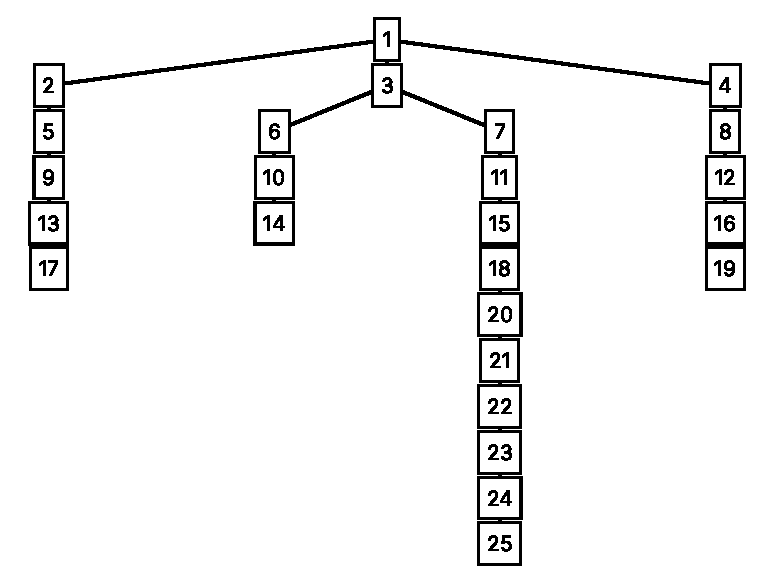
\includegraphics[width=0.6\textwidth]{figures/fig3_tree.pdf}
\caption{The tree of levels (\code{plot_branch_tree}). Each box is a level, labelled by its
\code{name}; lines join a level to the levels grown from it. Level 1 splits into 2, 3 and 4, and
level 3 into 6 and 7. The labels coincide with those printed by Kinnear's \code{render_tree}.}\label{fig:tree}
\end{figure}

\begin{figure}[p]
\centering
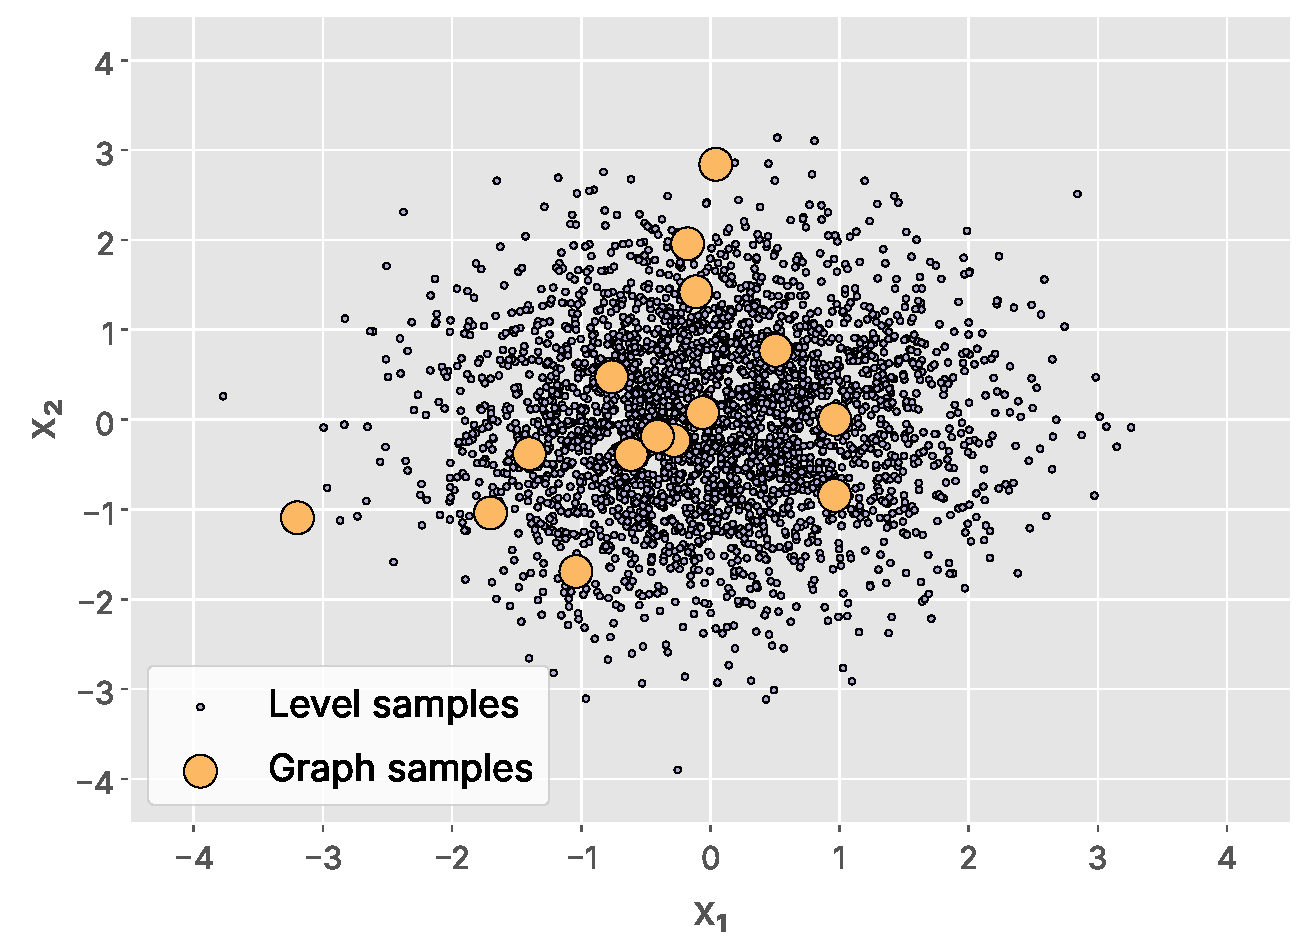
\includegraphics[width=0.48\textwidth]{figures/fig4_graph_samples.pdf}\hfill
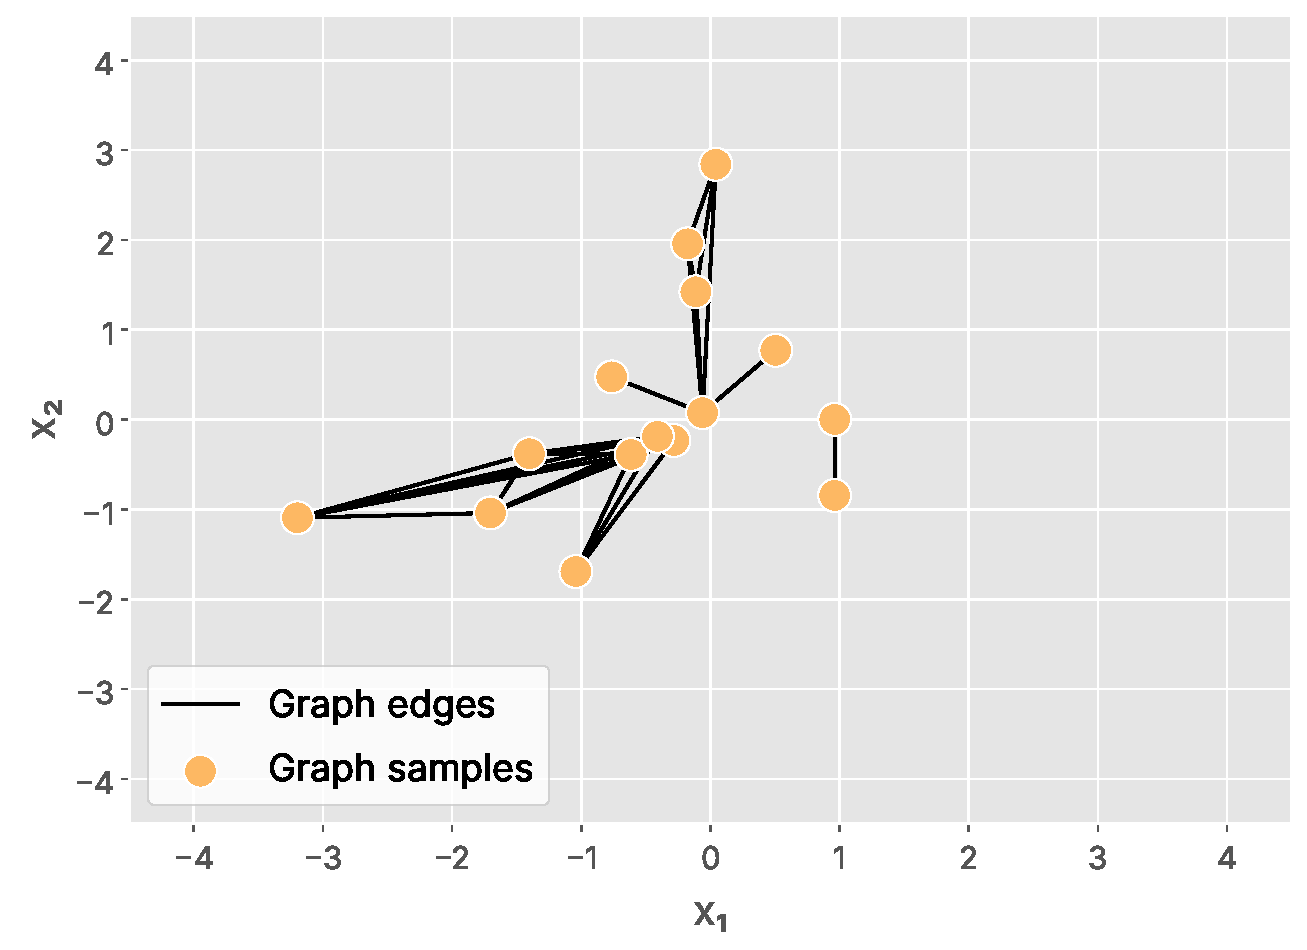
\includegraphics[width=0.48\textwidth]{figures/fig5_hvg.pdf}
\caption{Left: all samples of level 1 and the graph samples chosen in Stage 1. Right: the hill valley
graph of Stage 2 (Kinnear's \code{partitioner.py}).}\label{fig:graphsamples}
\end{figure}

\begin{figure}[p]
\centering
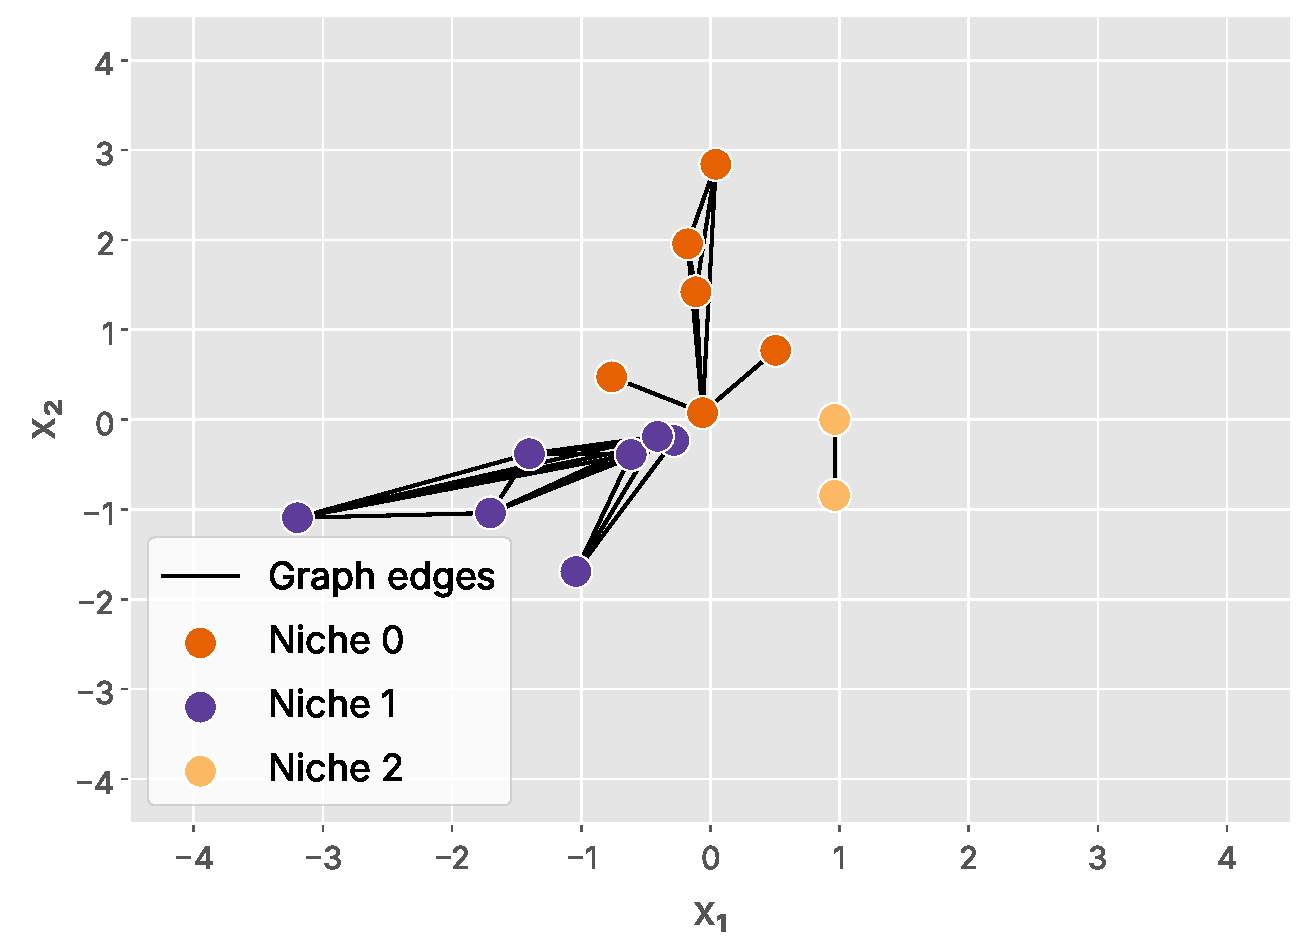
\includegraphics[width=0.48\textwidth]{figures/fig6_communities.pdf}\hfill
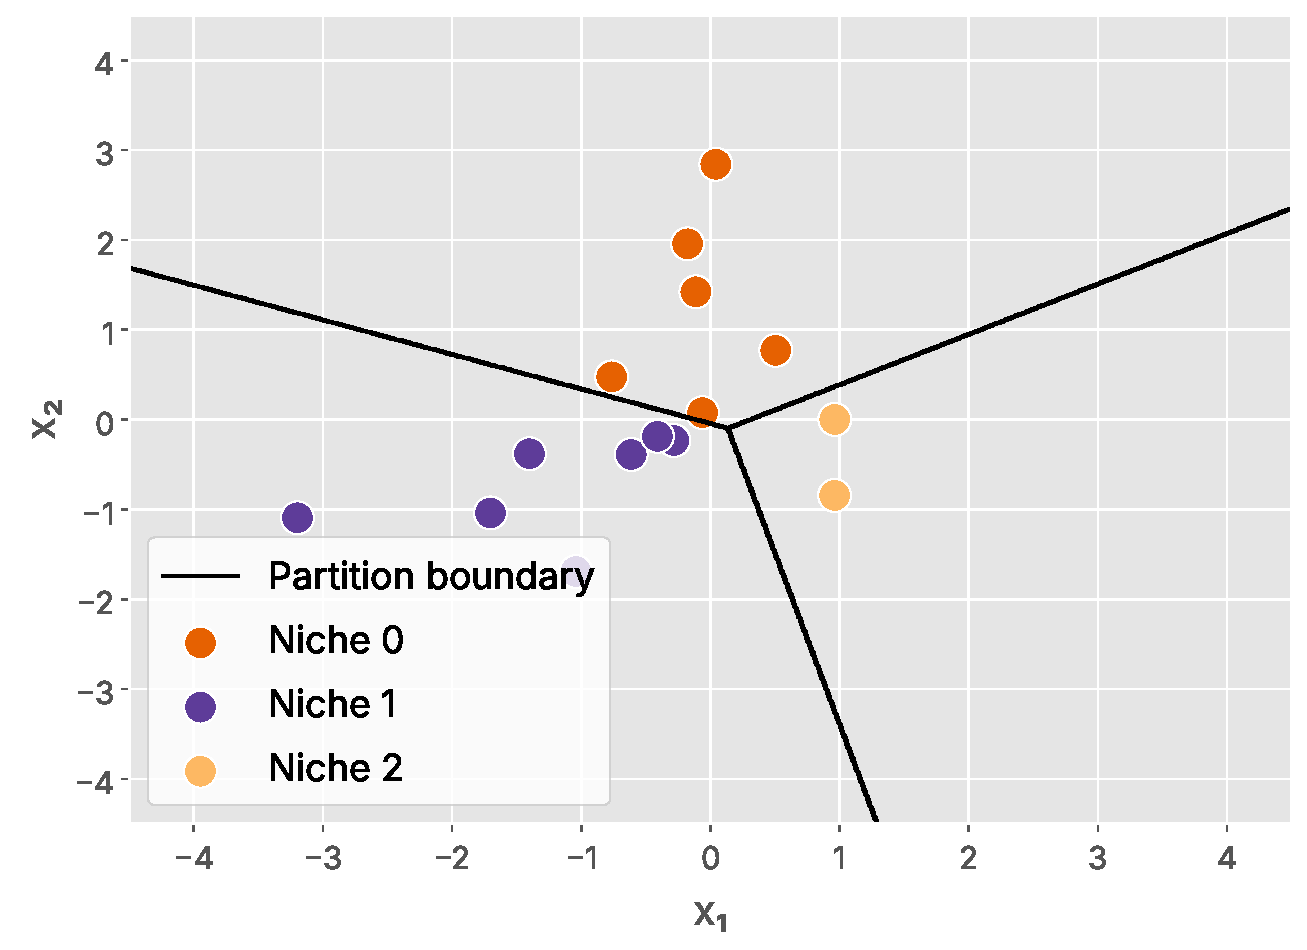
\includegraphics[width=0.48\textwidth]{figures/fig7_classifier.pdf}
\caption{Left: communities found in Stage 3. Right: the partition defined by the classifier of
Stage 4.}\label{fig:classifier}
\end{figure}

\clearpage

%=====================================================================
\section{The run block and its output}\label{sec:run}
%=====================================================================

The run block (i) computes the reference value~\eqref{eq:chi2}; (ii) runs \code{subset_simulation};
(iii) builds and runs \code{HillValleyGraphNSuS} with the parameters of Section~\ref{sec:setup};
(iv) prints $\hat p_F$, the number of levels and branches and the cost; (v) draws the figures. For
the parameters above the output is

\begin{lstlisting}[language={}]
SUBSET SIMULATION
Conditional levels L : 4
Total samples N      : 13800
pF (subset sim)      : 4.1567e-05

Level 1 partitioned into 3.
Level 3 partitioned into 2.
Failure stopper has stopped level 14.
Failure stopper has stopped level 17.
Failure stopper has stopped level 19.
Threshold Converge stopper has stopped level 25.
No more options, algorithm terminated.

NICHING SUBSET SIMULATION
Levels / branches    : 25 / 4
Total samples N      : 11644  (0 for hill valley graphs)
pF (NSuS)            : 2.4313e-05

pF (true value)      : 4.5400e-05
\end{lstlisting}

The costs are counted differently: subset simulation counts $n(1-p)$ new samples per level, NSuS
counts distinct evaluations. No midpoint evaluations were needed because, with $n = 3000$, every
box $Q_{ij}$ already contained stored points. The ending of each branch can be printed with
\begin{lstlisting}
for leaf in nss.leaves:
    ended = [k for k, v in leaf.stop_info.items() if v]
    print(f"branch ending at level {leaf.name}: {ended}, "
          f"pF contribution = {estimate_leaf_probability(YF, leaf):.3e}")
\end{lstlisting}

%=====================================================================
\section{Changing the problem and the parameters}\label{sec:change}
%=====================================================================

\subsection{Parameters}

\begin{table}[H]
\centering\small
\begin{tabularx}{\textwidth}{@{}l l Y@{}}
\toprule
Parameter & Value & Effect of increasing it \\
\midrule
$d$ & 2 & higher dimension; figures only for $d = 2$ \\
$Y_F$ & 20 & rarer event, more levels, smaller $p_F$ \\
$n$ & 3000 & lower variance, higher cost; $np$ and $1/p$ must be integers \\
$p$ & 0.1 & fewer, larger steps \\
\code{SEED} & 0 & any integer reproduces a run; \code{None} gives a new run \\
\code{GRAPH_SIZE} & 15 & more reliable niche detection, slightly more cost \\
\code{MAX_BRANCHES} & 4 & more regions followed at once; $1$ gives subset simulation \\
\code{SCALE} & 1.0 & larger proposal steps, lower acceptance; \code{None} is adaptive \\
\bottomrule
\end{tabularx}
\caption{Parameters and their effect.}
\end{table}

\subsection{Performance functions}

Any $g$ may be used provided it accepts a $(d, N)$ array and a single point, and failure is $g \ge Y_F$;
write it with \code{x[0]}, \code{x[1]} and NumPy functions. With each new $g$ change $Y_F$ and the
reference value \code{pF}.

\paragraph{Piecewise linear}~\cite{kinnear}, $Y_F = 0$, reference $p_F = 3.18\times10^{-5}$:
\begin{gather}
g(\x) = -\min\big(g_1(x_1), g_2(x_2)\big), \\
g_1(x_1) = \begin{cases} 4 - x_1 & x_1 > 3.5, \\ 0.85 - 0.1x_1 & \text{otherwise}, \end{cases} \qquad
g_2(x_2) = \begin{cases} 0.5 - 0.1x_2 & x_2 > 2, \\ 2.3 - x_2 & \text{otherwise}. \end{cases}
\end{gather}
\begin{lstlisting}
def performance_function(x):
    g1 = np.where(x[0] > 3.5, 4 - x[0], 0.85 - 0.1 * x[0])
    g2 = np.where(x[1] > 2, 0.5 - 0.1 * x[1], 2.3 - x[1])
    return -np.minimum(g1, g2)
\end{lstlisting}

\paragraph{Mixture of four bumps}~\cite{kinnear}, $Y_F = 0$, reference $p_F = 2.19\times10^{-4}$:
\begin{equation}
g(\x) = \frac{1}{2\pi}\sum_{i=1}^{4} w_i \exp\!\Big(-\tfrac12\|\x - \bm{\mu}_i\|^2\Big) - 0.04,
\end{equation}
with $\bm{\mu} = (3,3), (2,-2), (-2,2), (-2,-2)$ and $w = (0.4, 0.2, 0.2, 0.2)$.
\begin{lstlisting}
def performance_function(x):
    x = np.asarray(x, dtype=float)
    means = [(3, 3), (2, -2), (-2, 2), (-2, -2)]
    weights = [0.4, 0.2, 0.2, 0.2]
    total = 0
    for w, (m1, m2) in zip(weights, means):
        total = total + w * np.exp(-0.5 * ((x[0] - m1)**2 + (x[1] - m2)**2))
    return total / (2 * np.pi) - 0.04
\end{lstlisting}

\paragraph{Functions with exact answers.}
\begin{equation}
\begin{aligned}
g &= x_1 + x_2,                       & Y_F &= 5,   & p_F &= \Phi(-5/\sqrt2), \\
g &= |x_1|,                            & Y_F &= 3.5, & p_F &= 2\Phi(-3.5), \\
g &= \max(|x_1|, |x_2|),               & Y_F &= 3.5, & p_F &= 1 - \big(1 - 2\Phi(-3.5)\big)^2 .
\end{aligned}
\end{equation}

\subsection{Figures for a new problem}

Kinnear's \code{partitioner_figures} uses the fixed range $[-2, 3.2]\times[-4,4]$ unless one is passed, e.g.
\begin{lstlisting}
partitioner_figures(nss, split[0].name, x_range=(-4.5, 4.5), y_range=(-4.5, 4.5))
\end{lstlisting}
To colour up to four niches, replace the \code{zip} line in both places by
\begin{lstlisting}
for part_set,c,label in zip(sample_partition,[colors[0],colors[3],colors[1],colors[2]],['Niche 0','Niche 1','Niche 2','Niche 3']):
\end{lstlisting}

%=====================================================================
\section{Numerical experiments}\label{sec:experiments}
%=====================================================================

\subsection{Ring, $Y_F = 20$, $p_F = 4.54\times10^{-5}$}

\begin{table}[H]
\centering\small
\begin{tabular}{@{}lcccc@{}}
\toprule
Change from Section~\ref{sec:setup} & $\hat p_F^{\,\mathrm{NSuS}}$ & $N$ & Levels & Branch endings \\
\midrule
none & $2.43\times10^{-5}$ & 11644 & 25 & F F X F \\
\code{MAX_BRANCHES = 1} & $3.78\times10^{-5}$ & 12452 & 5 & F \\
\code{MAX_BRANCHES = 2} & $5.05\times10^{-5}$ & 11770 & 9 & F F \\
\code{GRAPH_SIZE = 30} & $3.04\times10^{-5}$ & 11425 & 26 & X F F F \\
\code{SCALE = None} & $4.02\times10^{-5}$ & 11946 & 19 & F F F F \\
$n = 1000$ & $2.77\times10^{-5}$ & 3823 & 20 & F F F F \\
\bottomrule
\end{tabular}
\caption{Single runs, \code{SEED = 0}. F: branch reached failure; X: stopped by ThresholdConverge.}
\end{table}

\begin{table}[H]
\centering\small
\begin{tabular}{@{}cccc@{}}
\toprule
$Y_F$ & exact $p_F$ & $\hat p_F^{\,\mathrm{SS}}$ & $\hat p_F^{\,\mathrm{NSuS}}$ \\
\midrule
20 & $4.54\times10^{-5}$ & $4.16\times10^{-5}$ & $2.43\times10^{-5}$ \\
25 & $3.73\times10^{-6}$ & $2.80\times10^{-6}$ & $1.14\times10^{-6}$ \\
30 & $3.06\times10^{-7}$ & $1.82\times10^{-7}$ & $8.50\times10^{-8}$ \\
\bottomrule
\end{tabular}
\qquad
\begin{tabular}{@{}lccc@{}}
\toprule
20 seeds, $n = 1000$ & mean $\hat p_F$ & CoV & mean $N$ \\
\midrule
SuS & $4.99\times10^{-5}$ & 0.78 & 4465 \\
NSuS, 1 branch & $4.39\times10^{-5}$ & 0.51 & 4118 \\
NSuS, 4 branches & $4.75\times10^{-5}$ & 0.74 & 3779 \\
\bottomrule
\end{tabular}
\caption{Left: rarer events, \code{SEED = 0}, $n = 3000$. Right: repeated runs.}
\end{table}

The ring is a single connected failure region. NSuS nevertheless splits it into angular sectors,
each sector receives a smaller share of the budget, and one sector frequently stalls. Over repeated
runs all three estimators are close to the exact value with comparable scatter: niching offers no
advantage here.

\subsection{Piecewise linear, $Y_F = 0$, $p_F = 3.18\times10^{-5}$}

\begin{table}[H]
\centering\small
\begin{tabular}{@{}lccc@{}}
\toprule
Change from Kinnear's example & $\hat p_F^{\,\mathrm{NSuS}}$ & $N$ (hill valley) & Levels / branches \\
\midrule
none & $1.83\times10^{-5}$ & 2421 (6) & 10 / 2 \\
\code{MAX_BRANCHES = 1} & $3.18\times10^{-7}$ & 2881 (0) & 7 / 1 \\
\code{GRAPH_SIZE = 6} & $5.72\times10^{-5}$ & 2567 (2) & 11 / 2 \\
\code{GRAPH_SIZE = 30} & $5.94\times10^{-5}$ & 2440 (38) & 10 / 2 \\
\code{SCALE = None} & $4.48\times10^{-5}$ & 2990 (5) & 12 / 2 \\
\code{MAX_BRANCHES = 4} & $3.97\times10^{-5}$ & 2174 (10) & 19 / 4 \\
\bottomrule
\end{tabular}
\caption{Kinnear's example: $n = 500$, \code{SEED = 2}, \code{GRAPH_SIZE = 14}, \code{MAX_BRANCHES = 2}.}
\end{table}

Without splitting the run follows only the more accessible failure region and misses the region
$\{x_1 \ge 4, x_2 \le 2\}$, underestimating $p_F$ by two orders of magnitude. With two branches both regions
are followed. Over 100 runs Kinnear reports that subset simulation misses this region in $65\%$ of runs
and NSuS in $2\%$~\cite{kinnear}. Niching is beneficial when the failure domain consists of genuinely
separate regions.

%=====================================================================
\section{Troubleshooting}\label{sec:trouble}
%=====================================================================

\begin{table}[H]
\centering\small
\begin{tabularx}{\textwidth}{@{}Y Y@{}}
\toprule
Symptom & Remedy \\
\midrule
\code{TypeError} in \code{ModifiedMetropolis.__init__} & a class was pasted inside another; each class must appear once \\
\code{NameError} for a function & save the file; keep every \code{def} above the run block \\
\code{NameError: plt} & keep \code{import matplotlib.pyplot as plt} at the top \\
tuple errors inside $g$ & pass \code{lambda x: performance_function(np.array(x))} \\
\code{ValueError: n*p and 1/p must be integers} & use $n$ a multiple of 10 for $p = 0.1$ \\
program never finishes & guard subset simulation: \code{while nF[L] / n < p and L < 30:} \\
\code{RecursionError} & \code{sys.setrecursionlimit(10000)} \\
points outside Figures~\ref{fig:graphsamples}--\ref{fig:classifier} & pass \code{x_range}, \code{y_range} \\
\code{KeyError} in \code{partitioner_figures} & name a level that was split \\
$\hat p_F = 0$ & no branch reached $Y_F$: increase $n$ or \code{MAX_BRANCHES}, or change \code{SEED} \\
\bottomrule
\end{tabularx}
\end{table}

\begin{thebibliography}{9}
\bibitem{aubeck} S.-K. Au and J.~L. Beck, Estimation of small failure probabilities in high dimensions
by subset simulation, \emph{Probabilistic Engineering Mechanics} 16(4):263--277, 2001.
\bibitem{kinnear} H. Kinnear, \emph{Niching subset simulation}, with companion code at
\url{https://github.com/HughKinnear/nsus_paper}.
\end{thebibliography}

\end{document}
